
\section{Extraction of Classes}
\label{sec:kgqa_extraction_of_classes}

A total of 81 publications were considered in our literature survey in the first ($\mathcal{L}_1$) and second ($\mathcal{L}_2$) iterations. Among these publications, 27 were selected as sources for class extraction ($\mathcal{F}$). After the search, we performed a manual extraction of the classes. A total of 227 classes were extracted from these publications. 

In the following sections, we analyze the distribution of the classes and publications from which the classes have been extracted. We first look at the distribution of the classes by the category and domain of the publication. Subsequently, we analyze the publication years prior to evaluating the citations and references among the papers.

\subsection{Distribution of Classes by Category and Domain}

\begin{table}[t]
    \centering
    \begin{tabular}{l l r r}
        \toprule
        \textbf{Category} & \textbf{Domain} & \textbf{Classes} & \textbf{Papers} \\
        \midrule
        KGQA Dataset & General & 27 & 4 \\
        KGQA Dataset & Requirements Engineering & 3 & 1 \\
        KGQA Dataset & Scholarly & 38 & 4 \\
        KGQA Dataset & Covid & 9 & 1 \\
        Question Classifier & General & 58 & 6 \\
        Question Classifier & Social Science & 4 & 1 \\
        Question Classifier & Spoken NLP & 8 & 1 \\
        Question Classifier & Vietnamese Language & 22 & 1 \\
        Research Questions & General & 12 & 2 \\
        Research Questions & Design Science & 10 & 1 \\
        Research Questions & Software Engineering & 21 & 2 \\
        Research Questions & Healthcare & 3 & 1 \\
        Other & General & 8 & 1 \\
        Other & Software Engineering & 4 & 1 \\
        Total & & 227 & 27 \\
        \bottomrule
    \end{tabular}
    \caption[Distribution of Classes by Paper Category and Domain]{Distribution of the extracted classes by the papers they were extracted from.}
    \label{table:question_type_distribution}
\end{table}

During the search, we assigned each paper to one of the categories introduced in the planning step. If a paper could not be clearly classified into any of the predefined categories, we added it to the category \emph{Other}. Furthermore, each publication was assigned a domain to understand its scope. 

\autoref{table:question_type_distribution} shows the distribution of the publications and extracted classes based on these categories and domains. The table illustrates that most of the question classes come from the category \emph{Question Classifier}, which includes those publications that propose methods to classify questions. This category comprises 92 question classes sourced from nine publications in four domains. Most of the papers in this category fall into the General domain, which means that their classifications are not limited to a specific topic area. Each of the remaining domains in this category (Social Science, Spoken NLP, Vietnamese Language) is represented by only a single paper. It is logical that this category includes the largest number of classes, as considering question structure and types is crucial when building classifiers. The classes extracted from these papers primarily relate to a form of answer type in which the expected format and content of the answer are considered, and the types of questions, which reflects the data processing required to derive an answer.

The second largest category by number of extracted classes is the \emph{\gls{kgqa} Dataset} category (77 classes from 10 papers). This category includes papers that propose a dataset for \gls{kgqa} and is represented by four domains, where the General domain and the Scholarly domain are equally represented by four papers each. The other two domains covered are Requirements Engineering, and one paper related to Covid. In general, this category provides critical insights relevant when working with \glspl{kg}. The literature suggests considering the structure of the \gls{kg} when classifying questions, which can indicate the complexity of the retrieval task. Additionally, considering the required \gls{kg} operations is relevant for understanding processing needs.

The third most common category is \emph{Research Questions}, which includes publications focused on the formulation and structure of research questions. Represented by six papers, this category includes 46 extracted question classes from four different domains. The General and Software Engineering domains are equally represented, each with two papers. The other two domains are related to Design Science and Healthcare. Generally, this category is useful for understanding the needs of researchers, which is particularly important for our taxonomy. As such, the literature highlights the importance of considering the focus of a question and its intended goal.

Finally, the \emph{Other} category includes publications that did not fit the predefined categories. This category is represented by two papers and includes 12 extracted question classes. The domains of these papers are Software Engineering and the General domain.

\subsection{Distribution of Publications by Year}

\begin{figure}[t]
    \centering
    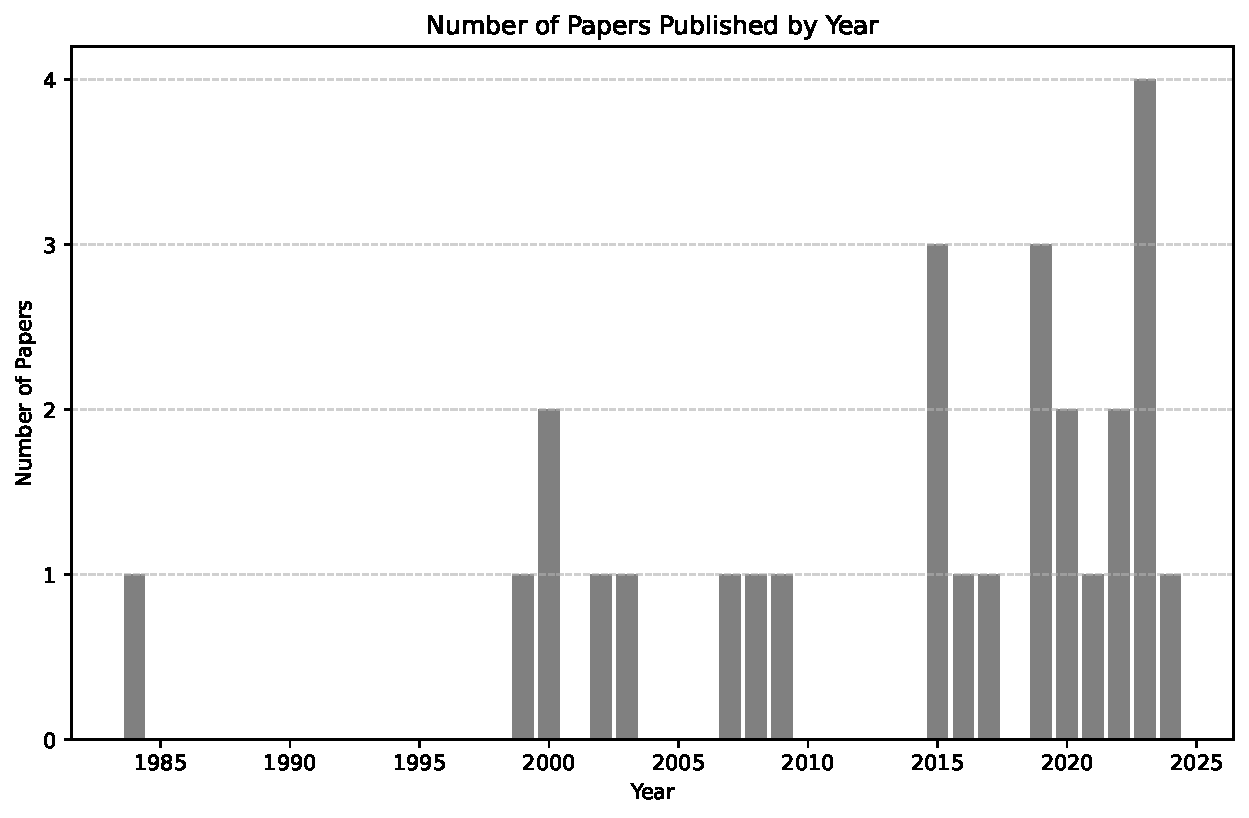
\includegraphics[width=0.99\textwidth]{figures/question_catalog/papers_by_year.pdf}
    \caption[Distribution of Papers by Publication Year]{The distribution of papers by their year of publication.}
    \label{fig:papers_by_year}
\end{figure}

\autoref{fig:papers_by_year} shows the distribution by publication year for the papers from which we extracted classes. The years range from 1984 to 2024, with most publications published in the last decade. The oldest paper is authored by \textcite{dillon_classification_1984}, who investigated the classification of research questions as suggested by Aristotle. The most recent paper is authored by \textcite{taffa_hybrid-squad_2024}, which presents the Hybrid-SQuAD dataset designed to address scholarly \gls{qa} by combining tabular and textual data. The year 2023 yielded the most publications in our set (four papers), while other years contributed between one and three papers. Several years within the range had no publications matching our criteria.



\subsection{Distribution of Citations and References}

\begin{table}[t]
    \centering
    \begin{minipage}[t]{0.43\textwidth}
        \centering
        \begin{tabular}{l c}
            \toprule
            \textbf{Paper} & \textbf{Number of Citations} \\
            \midrule
            \cite{li_learning_2002} & \cite{auer_sciqa_2023}, \cite{bolotova_non-factoid_2022}, \cite{allam_question_2016}, \cite{chernov_linguistically_2015} \\
            \cite{dubey_lc-quad_2019} & \cite{auer_sciqa_2023}, \cite{usbeck_qald-10_2023}, \cite{banerjee_dblp-quad_2023} \\
            \cite{singhal_att_1999} & \cite{auer_sciqa_2023}, \cite{chernov_linguistically_2015} \\
            \cite{mikhailian_learning_2009} & \cite{auer_sciqa_2023}, \cite{chernov_linguistically_2015} \\
            \cite{auer_sciqa_2023} & \cite{karras_divide_2023}, \cite{taffa_hybrid-squad_2024} \\
            \cite{jaradeh_question_2020} & \cite{karras_divide_2023}, \cite{taffa_hybrid-squad_2024} \\
            \cite{bordes_large-scale_2015} & \cite{auer_sciqa_2023} \\
            \cite{riloff_rule-based_2000} & \cite{auer_sciqa_2023} \\
            \cite{sjoberg_future_2007} & \cite{karras_divide_2023} \\
            \cite{moldovan_structure_2000} & \cite{chernov_linguistically_2015} \\
            \cite{banerjee_dblp-quad_2023} & \cite{taffa_hybrid-squad_2024} \\
            \bottomrule
        \end{tabular}
        \caption[Number of Citations within Paper Selection]{The number of times a paper has been cited by another paper within $\mathcal{F}$.}
        \label{table:papers_by_citations}
    \end{minipage}
    \hfill
    \begin{minipage}[t]{0.55\textwidth}
        \centering
        \begin{tabular}{l c}
            \toprule
            \textbf{Paper} & \textbf{References} \\
            \midrule
            \cite{auer_sciqa_2023} & \cite{bordes_large-scale_2015}, \cite{dubey_lc-quad_2019}, \cite{li_learning_2002}, \cite{singhal_att_1999}, \cite{riloff_rule-based_2000}, \cite{mikhailian_learning_2009} \\
            \cite{chernov_linguistically_2015} & \cite{singhal_att_1999}, \cite{moldovan_structure_2000}, \cite{mikhailian_learning_2009}\\
            \cite{karras_divide_2023} & \cite{sjoberg_future_2007}, \cite{auer_sciqa_2023}, \cite{jaradeh_question_2020} \\
            \cite{taffa_hybrid-squad_2024} & \cite{auer_sciqa_2023}, \cite{banerjee_dblp-quad_2023}, \cite{jaradeh_question_2020} \\
            \cite{bolotova_non-factoid_2022} & \cite{li_learning_2002} \\
            \cite{allam_question_2016} & \cite{li_learning_2002} \\
            \cite{banerjee_dblp-quad_2023} & \cite{dubey_lc-quad_2019} \\
            \cite{usbeck_qald-10_2023} & \cite{dubey_lc-quad_2019} \\
            \bottomrule
        \end{tabular}
        \caption[Number of References within Paper Selection]{The number of times a paper has referenced another paper within $\mathcal{F}$.}
        \label{table:papers_by_references}
    \end{minipage}
\end{table}


\autoref{table:papers_by_citations} illustrates the frequency with which the papers in our selected set ($\mathcal{F}$) cite each other. This provides insight into the relative influence of each publication within our selection. In particular, \cite{li_learning_2002} is the most frequently cited paper, indicating a potentially greater influence within our selected set of papers. In addition, five papers are cited twice and five are cited once, suggesting a modest influence within the set. Of the 27 papers in the final list, 16 were not cited by any other paper within this set, suggesting that they have had limited direct influence on the classification schemes developed in the cited works within our collection.

In contrast, \autoref{table:papers_by_references} details how often each paper references other publications within our selection. This data reveals the extent to which the classifications may have been informed by prior work. According to the data, \cite{auer_sciqa_2023} stands out with six references, indicating that its classifications are heavily influenced by other publications on our list. Similarly, \cite{chernov_linguistically_2015} references four papers, while both \cite{karras_divide_2023} and \cite{taffa_hybrid-squad_2024} cite three publications each. In addition, four papers \cite{bolotova_non-factoid_2022,allam_question_2016,banerjee_dblp-quad_2023,usbeck_qald-10_2023} include only one reference. Overall, with only eight out of 27 papers referencing other works in the data, it appears that most of the publications derive their insights independently.
